\documentclass[a4paper, 10pt, final]{article}
\usepackage{bonde}

\def\mytitle{Signal and Image Processing 2010}
\def\mysubtitle{Handin of mandatory excercise 7}
\def\myauthor{Ulrik Bonde}
\def\mymail{\mailto{bonde@diku.dk}}
\def\mydate{\today}
\def\repository{\url{http://github.com/bonde/sip}}

\title{\mytitle}
\subtitle{\mysubtitle}

\author{\myauthor{} - \mymail}
\date{\mydate}

\hypersetup{
colorlinks,%
citecolor=black,%
filecolor=black,%
linkcolor=black,%
urlcolor=black,%
bookmarksopen=false,
pdftitle={\mytitle{} - \mysubtitle},
pdfauthor={\myauthor}
}

\begin{document}
\maketitle

\subsection*{Question 7.1}
In this assignment we should implement the Hough transform using two
different approaches. The final goal is to detect lines in the image
shown in fig. \ref{apple}.

\begin{figure}[h!]
    \centering
    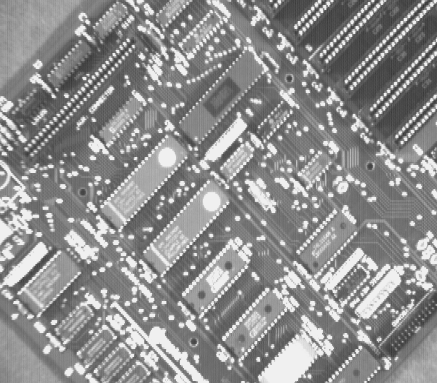
\includegraphics[angle=0,width=0.7\textwidth]{images/apple}
    \caption{Original image. Note that the image has a fair amount of
    noise, mostly periodic, vertical lines.}
    \label{apple}
\end{figure}

Only the Hough transform have been implemented. To find the
actual lines from the output of the Hough transform, the built-in
methods from the MATLAB image library called \texttt{houghpeaks} and
\texttt{houghlines} are used. \texttt{houghlines} is a very fancy method
that tries to find the actual line segment in the image. We are just
interested in the lines, so we avoid this behavior from MATLAB by
supplying an image filled with ones. This way MATLAB will believe that
everything in the image is an edge, and thus draw the entire line. When
\texttt{houghpeaks} is used we limit the number of peaks to 20. A note
on how to implement the above methods are included at the end of this
document.

Also, the Hough transform take an edge-detected image as input. For this
the Canny edge detection from MATLAB is used.

Finally the implementations calculate the structure tensor as the
supplied code from Jon Sporring and also use his method \texttt{scale}
for scaling and determining derivatives.

Before applying any operations the image will first have its colors
adjusted using the built-in \texttt{imadjust}.

\paragraph{1)}
The first implementation is only just mentioned in \citep[section
16.5.2, p. 458-460]{jahne-digital}. We use that a line can be
represented as
\begin{equation}
    x\cos\theta+y\sin\theta = \rho
\end{equation}
Now lines in the image can be represented in the parameter space by
their values of $\theta$ and $\rho$. We construct a $\rho\times\theta$
image which is called the Hough accumulator.

$\rho$ have values in the interval $[-D, D]$, where $D$ is the diagonal
of the image. The values of $\theta$ will normally be in the interval
$[-90, 90]$, but can be narrowed down to a more specific range of
degrees. However, my implementation use the fixed range of $[-90,90]$.
Using this we can allocate the array for the accumulator.

For each point of interest we then calculate $\rho$ using values of
$\theta$ ranging from -90 to 90 with a variable step size for precision
at a computational cost. For each computation of $\rho$ we then
increase the accumulator at the position $(\rho, \theta)$. Some rounding
of the $\rho$-values have to be done in order for them to fit into the
accumulator array.

Now every point in the original image corresponds to a sinusoid curve in
the accumulator. At the point in the accumulator where two curves
intersect means that these two points --- in the original image --- lies
on the same straight line. This line can be described by the $\rho$ and
$\theta$ values from the accumulator. An example is given in fig.
\ref{square_hough_transform}.

\begin{figure}[!h]
    \centering
    \subfloat[Original]{\label{square}
\includegraphics[angle=0,width=0.45\textwidth]{images/square}}\hspace{1em}
    \subfloat[Canny edge
    detection]{\label{square_edges}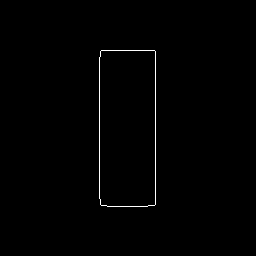
\includegraphics[angle=0,width=0.45\textwidth]{images/square_edges}}\\
    \subfloat[Hough
    transform. $x = \theta$, $y = \rho$]{\label{square_transform}
\includegraphics[angle=0,width=0.45\textwidth]{images/square_transform}}\hspace{1em}
    \subfloat[Found
    lines]{\label{square_lines}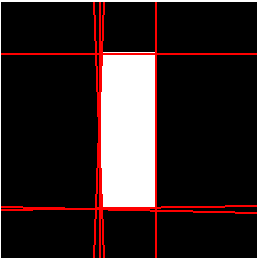
\includegraphics[angle=0,width=0.45\textwidth]{images/square_lines}}
    \caption[]{
    Hough transform of \texttt{square.tiff}.
    \textbf{Fig. \ref{square})} The original image in which
    we want to detect lines.
    \textbf{Fig. \ref{square_edges})} The edges found by Canny edge
    detection with a threshold of $0.4$ and $\sigma = 1.2$.
    \textbf{Fig. \ref{square_transform})} The Hough transform of the
    edges. $\theta$ have values in the interval $[-90,90]$ with four
    steps per degree, i.e. step size $0.25$. Note that we see four peaks
    (edges wrap) corresponding to the four lines in the original. We
    also have four clear traces of sinusoids.
    \textbf{Fig. \ref{square_lines})} The lines found by the built-in
    methods in MATLAB.
    }
    \label{square_hough_transform}
\end{figure}

In fig. \ref{apple_hough_transform} the Hough transform is applied to
the image in fig. \ref{apple}. In the Hough transform we see that the
peaks are grouped around two values of $\theta$ suggesting parallel
lines in the image just as in fig. \ref{square_hough_transform}. The
x-axis are $\theta$-values ranging from $-90\degree$ to $90\degree$ and
from this we see that the peaks are concentrated around $-45\degree$ and
$45\degree$. This seems fair considering the original image.

\begin{figure}[!h]
    \centering
    \subfloat[Canny edge
    detection]{\label{apple_edges}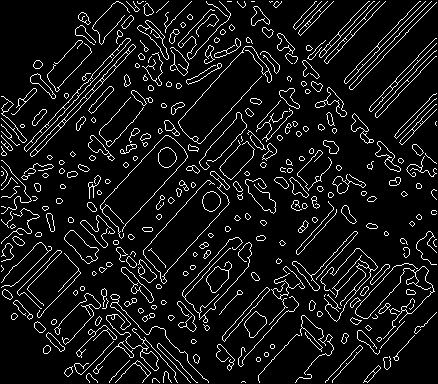
\includegraphics[angle=0,width=0.45\textwidth]{images/apple_edges}}\hspace{1em}
    \subfloat[Found
    lines]{\label{apple_lines}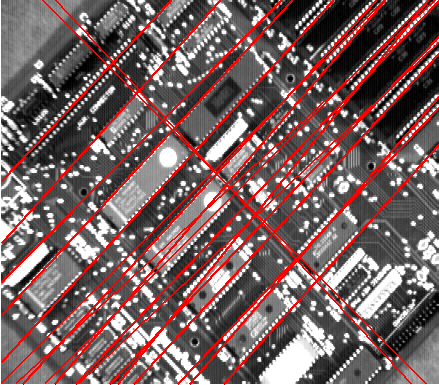
\includegraphics[angle=0,width=0.45\textwidth]{images/apple_lines}}\\
    \subfloat[Hough
    transform. $x = \theta$, $y = \rho$]{\label{apple_transform}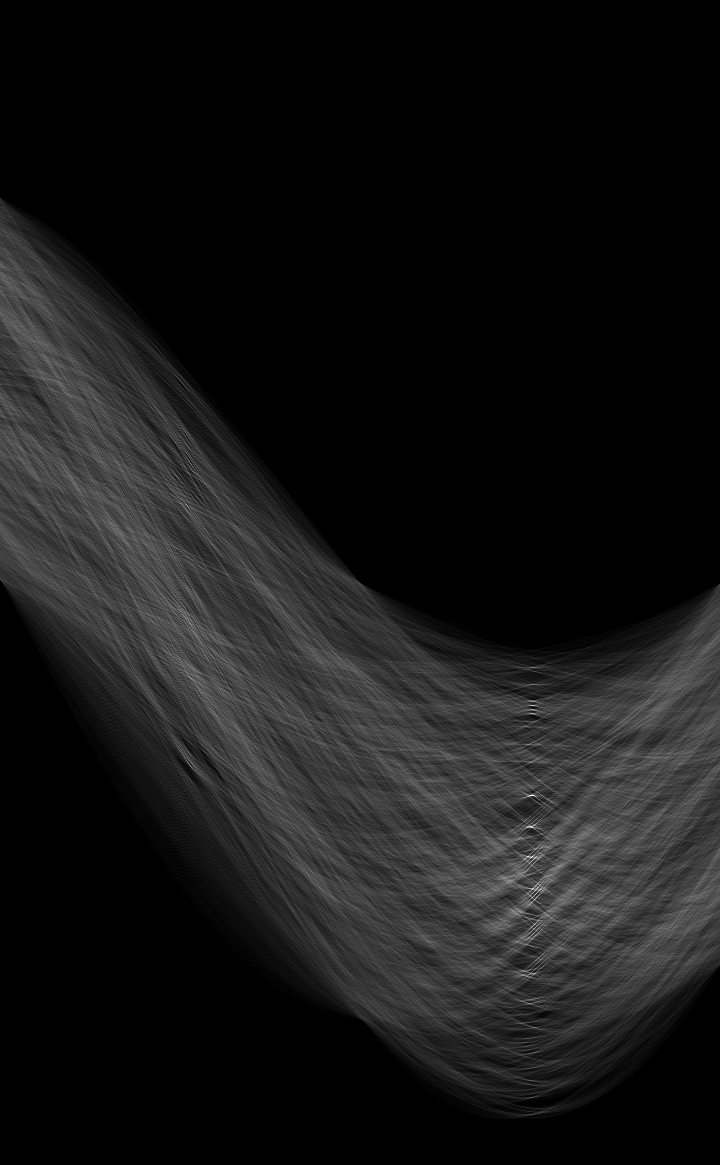
\includegraphics[angle=0,width=0.45\textwidth]{images/apple_transform}}
    \caption[]{
    Hough transform of \texttt{apple.tiff}.
    \textbf{Fig. \ref{apple_edges})} The edges found by Canny edge
    detection with a threshold of $0.4$ and $\sigma = 1.2$.
    \textbf{Fig. \ref{apple_lines})} The lines found by the built-in
    methods in MATLAB.
    \textbf{Fig. \ref{apple_transform})} The Hough transform of the
    edges with same $\theta$ as fig. \ref{square_hough_transform}. We
    see that we have two ``groups'' of peaks at two different values of
    $\theta$. This corresponds to the two major directions in the image.
    }
    \label{apple_hough_transform}
\end{figure}

\paragraph{2)}
The above method for the Hough transform is computationally expensive,
thus we want to speed up the transform. For this we can use the
structure tensor as it give the angle of the local neighbourhood. We
must note that the found lines will now depend on the structure tensor
and the arguments passed to the computation of this.

Study figure \ref{f_apple_hough_transform} for the result.

\begin{figure}[!h]
    \centering
    \subfloat[Structure tensor]{\label{f_apple_tensor}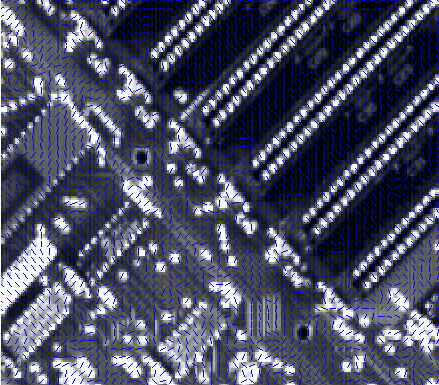
\includegraphics[angle=0,width=0.45\textwidth]{images/f_apple_tensor}}\hspace{1em}
    \subfloat[Found
    lines]{\label{f_apple_lines}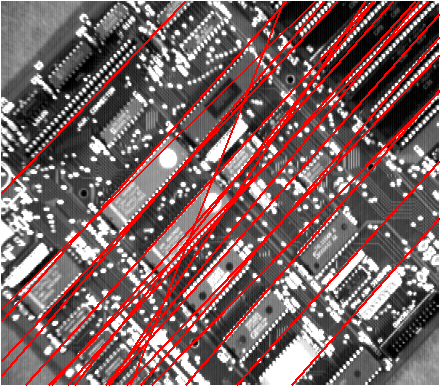
\includegraphics[angle=0,width=0.45\textwidth]{images/f_apple_lines}}\\
    \subfloat[Hough
    transform. $x = \theta$, $y =
    \rho$]{\label{f_apple_transform}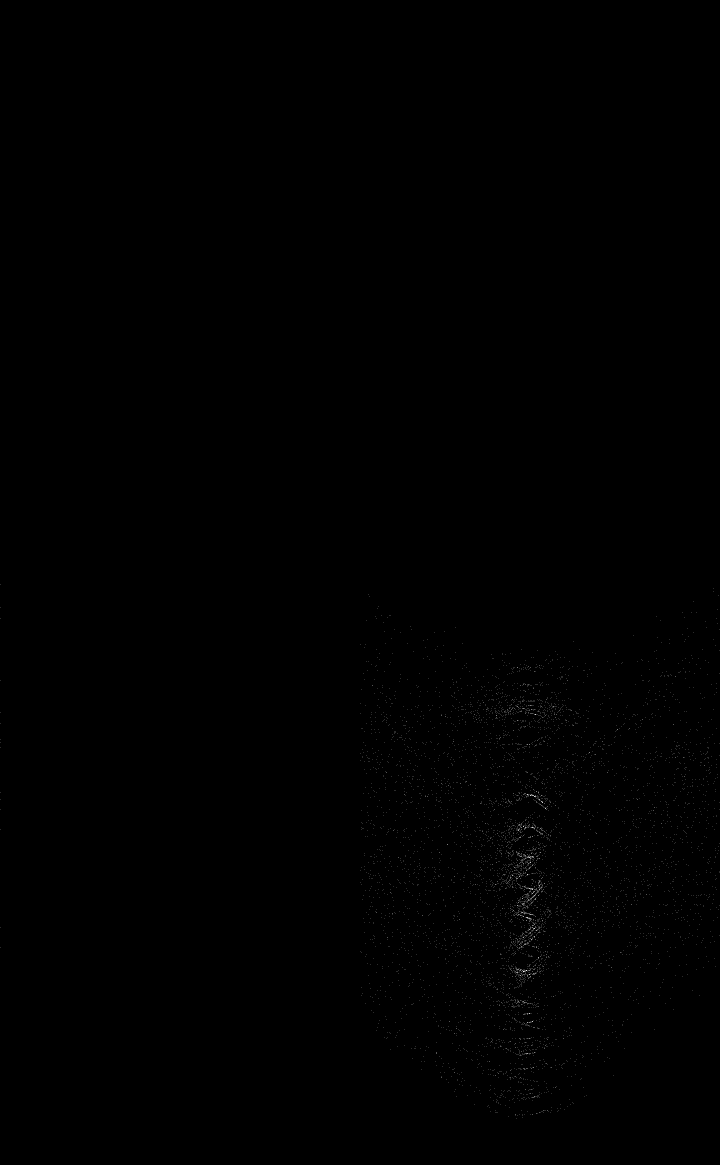
\includegraphics[angle=0,width=0.45\textwidth]{images/f_apple_transform}}
    \caption[]{
    Fast Hough transform of \texttt{square.tiff}.
    \textbf{Fig. \ref{f_apple_tensor})} The structure tensor on the
    original image with $\sigma_1 = 1$ and $\sigma_2 =
    2$. The image is a zoom of the upper right corner.
    \textbf{Fig. \ref{f_apple_lines})} The lines we detect from the
    Hough transform. This is not as accurate as the previous transform.
    We have some false lines.
    \textbf{Fig. \ref{f_apple_transform})} The Hough accumulator. Notice
    that we do not detect any lines with an angle of $-45\degree$. The
    $\theta$-values are concentrated around $45\degree$.
    }
    \label{f_apple_hough_transform}
\end{figure}

\subsubsection*{Comparison}
We have seen that the first method is more precise in that we do not
observe any false lines. The fast Hough transform do detect some false
lines, but the results are somewhat trustworthy.

For some reason, the first method is better at finding different angles.
In fig. \ref{f_apple_hough_transform} we saw that the fast Hough
transform only found lines with almost the same angle. The fast Hough
transform \emph{is} able to detect different angles. This is
demonstrated in fig. \ref{f_R1_lines} in the image of the Pentagon. In
the images in fig. \ref{f_R1_lines} it is really hard to determine which
method is best. They do find some of the same lines, but are not
entirely the same. It does still apply that the first method finds more
different angles than the fast Hough transform.

In the images of the chip board the first method is most trustworthy.
In all the above the same arguments have been passed to the edge
detector, but the different scales used to find the structure tensor
also plays a big role. By tweaking these parameters --- as well as the
parameter to the edge detection --- one could probably find some better
results.

\begin{figure}[!h]
    \centering
    \subfloat[Hough
    transform]{\label{R1_lines}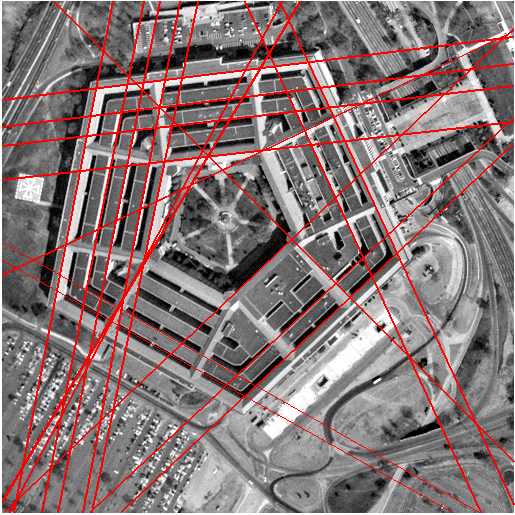
\includegraphics[angle=0,width=0.65\textwidth]{images/R1_lines}}\\
    \subfloat[Fast Hough
    transform]{\label{f_R1_lines}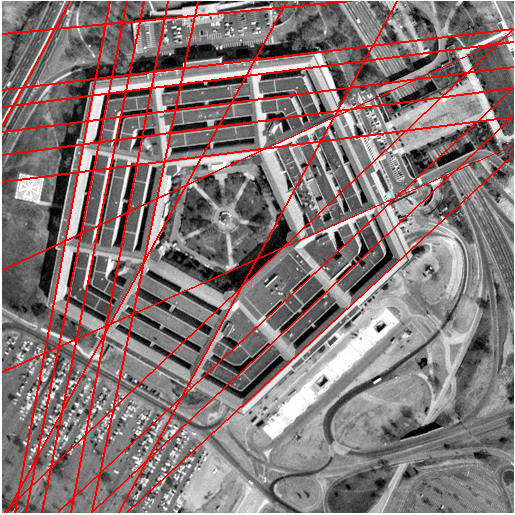
\includegraphics[angle=0,width=0.65\textwidth]{images/f_R1_lines}}
    \caption[]{
    Detected lines with the two methods in \texttt{R1.tiff}.
    \textbf{Fig. \ref{R1_lines})} The first method manages to outline
    the entire building by finding a line on each side of the pentagon
    structure. Only lines on the building are found.
    \textbf{Fig. \ref{f_R1_lines})} The fast Hough transform does not
    find a line on each side on the building, but does find some
    roads outside. No false lines are found.
    }
    \label{R1_hough_transform}
\end{figure}

\subsubsection*{Note on detection and determination of lines}
Given a Hough accumulator one wish to detect local maxima. This is where
the curves intersect and thus this represent point on the same line in
the image.

To find these maxima one can threshold the image leaving only pixels
above a certain level in the image. The coordinates of these peaks are
then returned.

With these positions we can find the value of $\rho$ and $\theta$ for
the lines. Then the lines can be plotted in the image.

\clearpage

%%%%%%%%%%%%%%%%%%%%%%%%%%%%%%%%%%%%%%%%%%%%%%%%%%%%%%%%%%%%%%%%%%%%
% Formal stuff

\bibliographystyle{abbrvnat}
\bibliography{bibliography}
%\addcontentsline{toc}{chapter}{Litteratur}

\appendix
\lstset{language=Matlab, basicstyle=\scriptsize,
    showstringspaces=false, numbers=left, stepnumber=1,
    numberstyle=\tiny, frame=none}
\section{Source code}
The full source can be viewed and downloaded from my repository at
\repository{}.

\subsection{SIPHoughTransform.m}
\lstinputlisting{../src/SIPHoughTransform.m}

\subsection{SIPFastHoughTransform.m}
\lstinputlisting{../src/SIPFastHoughTransform.m}

\subsection{AltTensor.m}
\lstinputlisting{../src/AltTensor.m}

\end{document}

% vim: set tw=72 spell spelllang=en:
